\documentclass{estilo}
\usepackage[spanish]{babel}
\usepackage{graphicx}
\usepackage{float}
\usepackage{amsmath}        % para los vectores columnas
\usepackage{amsfonts}       % para las negrita de pizarra
\usepackage{amssymb}        % para simbolos matematicos
\usepackage{hyperref}       % para utilizar referencias
\usepackage{multirow}       % para las tablas
\usepackage{dsfont}
\usepackage{listings}
\usepackage{xcolor}
\definecolor{codegreen}{rgb}{0,0.6,0}
\definecolor{codegray}{rgb}{0.5,0.5,0.5}
\definecolor{codepurple}{rgb}{0.58,0,0.82}
\definecolor{backcolour}{rgb}{0.95,0.95,0.92}
\lstdefinestyle{mystyle}{
    backgroundcolor=\color{backcolour},   
    commentstyle=\color{codegreen},
    keywordstyle=\color{magenta},
    numberstyle=\tiny\color{codegray},
    stringstyle=\color{codepurple},
    basicstyle=\ttfamily\footnotesize,
    breakatwhitespace=false,         
    breaklines=true,                 
    captionpos=b,                    
    keepspaces=true,                 
    numbers=left,                    
    numbersep=5pt,                  
    showspaces=false,                
    showstringspaces=false,
    showtabs=false,                  
    tabsize=2
}
\lstset{style=mystyle}

\usepackage{enumitem,multicol,setspace}
\newcounter{subenum}[enumi] % para las multicolumnas
\renewcommand{\thesubenum}{\arabic{subenum}}
\usepackage[nomessages]{fp}
\FPeval\thecolwidth{round(1/4:4)}% Specify number of columns -> column width
\newcommand{\newitem}[1]{%
  \refstepcounter{subenum}%
  \parbox{\dimexpr\thecolwidth\linewidth-.5\columnsep}{%
    \makebox[\labelwidth][r]{(\thesubenum)\hspace*{\labelsep}}%
    #1}\hfill%
}

\usepackage{scalerel,stackengine} % para el sombrero
\stackMath
\newcommand\rhat[1]{%
\savestack{\tmpbox}{\stretchto{%
  \scaleto{%
    \scalerel*[\widthof{\ensuremath{#1}}]{\kern-.6pt\bigwedge\kern-.6pt}%
    {\rule[-\textheight/2]{1ex}{\textheight}}%WIDTH-LIMITED BIG WEDGE
  }{\textheight}% 
}{0.5ex}}%
\stackon[1pt]{#1}{\tmpbox}%
}
\parskip 1ex

\usepackage{mathtools}      % floor y ceil
\DeclarePairedDelimiter\ceil{\lceil}{\rceil}
\DeclarePairedDelimiter\floor{\lfloor}{\rfloor} 

\usepackage[style=authoryear-comp]{biblatex}

\begin{document}
\maketitle
\newpage
\vspace*{\fill}
\begin{center}
\begin{quote}
\begin{flushright}
  "\textit{A la Selección Argentina, porque trajeron la tercera}" \\
  "\textit{A Lionel Scaloni, esta va con toda la intención de ayudarte}" \\
\end{flushright}
\end{quote}
\end{center}
\vspace*{\fill}
\newpage
\input{tex/1_reference}
\newpage
\section{El problema}
Scaloni ya está armando la lista de 43 jugadores que van a ir al mundial 2026. 
Hay mucha presión por parte de la prensa para bajar línea de cuál debería ser 
el 11 inicial. Lo de siempre. 
Algunos medios quieren que juegue Roncaglia, otros quieren que juegue 
Mateo Messi, y así. Cada medio tiene un subconjunto de
jugadores que quiere que jueguen. A Scaloni esto no le importa, no va a dejar
que la prensa lo condicione, pero tiene jugadores jóvenes a los que esto
puede afectarles. 

Justo hay un partido amistoso contra Burkina Faso la semana que viene. Oportunidad
ideal para poner un equipo que contente a todos, baje la presión y poder 
aislar al equipo. 

El problema es, ¿cómo elegir el conjunto de jugadores que jueguen ese partido 
(entre titulares y suplentes que vayan a entrar)? Además, Scaloni quiere poder
usar ese partido para probar cosas aparte. No puede gastar el amistoso
para contentar a un periodista mufa que habla mal de Messi, por ejemplo. 
Quiere definir el conjunto más pequeño de jugadores necesarios para contentarlos 
y poder seguir con la suya. Con elegir
un jugador que contente a cada periodista/medio, le es suficiente. 

Ante este problema, Bilardo se sentó con Scaloni para explicarle que en realidad 
este es un problema conocido (viejo zorro como es, ya se comió todas las operetas 
de prensa así que se conoce este problema de memoria). Se sirvió una copa de \textit{Gatorei} 
y le comentó:

Esto no es más que un caso particular del Hitting-Set Problem. El cual es: Dado un conjunto 
$A$ de $n$ elementos y $m$ subconjuntos $B_1, B_2, ..., B_m$ de $A$
($B_i \subseteq A \forall i$) , queremos el subconjunto $C \subseteq A$ de menor tamaño tal 
que $C$ tenga al menos un elemento de cada
$B_i$ (es decir, $C \cap B_i \neq \emptyset$). En nuestro caso, $A$ son los jugadores 
convocados, los $B_i$ son los deseos de la
prensa, y $C$ es el conjunto de jugadores que deberían jugar contra Burkina Faso 
si o si". 

Bueno, ahora con un poco más claridad en el tema, Scaloni necesita de nuestra 
ayuda para ver si obtener este subconjunto se puede hacer de forma eficiente 
(polinomial) o, si no queda otra, con qué alternativas contamos. 
\section{Estudiando Hitting Set Problem}

\subsection{Demostrando su pertenencia a NP}

Para demostrar que Hitting Set se encuentra en NP bastaría con tener una solución del problema: un conjunto $H$ y y el set de datos de entrada al mismo, un conjunto de subconjuntos $B = B_1, B_2, ... B_m$ ($B_i \subseteq A \forall i$) de manera que, simplemente, se debe iterar sobre el conjunto de subconjuntos y sobre cada subconjunto validando si alguno de los elementos $b_j \in B_i$ ciertamente pertenece a $H$. En caso de haber probado con todos los elementos de un $B_i$ y ninguno de sus elementos $b_j$ pertenezca a $H$ entonces, la solución brindada no es un Hitting Set, en caso de haber llegado al final entonces dicho conjunto si es un Hitting Set

\subsubsection{Implementación del validador}

\begin{lstlisting}[language=Python, caption= validador, label=python_code]
def is_solution(hitting_set, subsets):
    for subset in subsets:
        flag = False
        for element in subset:
            if element in hitting_set: 
                flag = True
                break
        if not flag: return False 
    return True
\end{lstlisting}

\subsubsection{Complejidad temporal del validador}

Para verificar finalmente que dicho problema falta con probar que este validador posee tiempo polinomial

Veamos que: 

\begin{itemize}
    \item Recorrer la lista de subconjuntos es lineal en la cantidad de subconjuntos, dicha cantidad se llamará $m$.
    \item Recorrer los elementos del subconjunto $B_i$ es lineal en la cantidad de elementos del subconjunto, dicha cantidad se llamará $k$.
\end{itemize}

Ahora si decimos generalizamos $k$ como el máximo cardinal existente de algún conjunto $B_i$ se puede establecer la siguiente cota:

$$
    T(n) = O(m \times k)
$$

Como dicha complejidad es polinomial a $m$ y $k$ entonces se cumple que Hitting Set esta  en NP

\subsection{Demostrando pertenece a NP completo}

Para probar este segmento del informe se debe realizar una reduccion de algun problema NP-Completo conocido a Hitting-Set, en este caso, dicho problema sera Vertex Cover.

En un principio se establecen ambos problemas de decisión: 

\begin{center}
  \begin{minipage}{0.8\textwidth}
    \fbox{%
      \parbox{\dimexpr\linewidth-2\fboxsep-2\fboxrule}{%
        \textbf{El problema de decisión del vertex cover implica, dado un grafo G y un número k, determinar si existe un vertex cover de tamaño a lo sumo k \\}
      }%
    }
  \end{minipage}
\end{center}

Por otro lado: 

\begin{center}
  \begin{minipage}{0.8\textwidth}
    \fbox{%
      \parbox{\dimexpr\linewidth-2\fboxsep-2\fboxrule}{%
        \textbf{El problema de decisión del hitting set implica, sea A un conjunto, B un conjunto de subconjuntos pertenecientes a A, determinar si existe un conjunto H de tamaño al menos k tal que todo subconjunto de B la intersección entre $B_i$ y H no es vacía \\}
      }%
    }
  \end{minipage}
\end{center}

Entonces veamos la siguiente reducción:

$$
    \text{Vertex Cover} \leq_p \text{Hitting Set} 
$$

Sea $G$ un grafo, $V$ su conjunto de vertices y $E$ su conjunto de aristas, entonces se toma $A$ como el conjunto de vertices. Ahora, que sera $B$, en este caso se podria definir como el conjunto de subconjunto de los pares $(v_i, v_j)$ siempre y cuando exista una arista entre dichos vertices, aunque, esto seria simplemente el conjunto de las aristas de $G$

Habiendo establecido lo anterior, se puede observar que si existe un Hitting Set de tamaño k  para los conjuntos $A = V(G)$ y $B = E(G)$ entonces necesariamente existe un vertex cover de tamaño al menos k, por lo tanto, sabiendo que vertex cover es un problema NP-Completo se puede concluir finalmente que Hitting set también es NP-Completo 

\newpage
\section{Implementando una solución}

Para implementar alguna solución exacta del problema dado lo probado en la sección anterior, es decir, la pertenencia del problema a conjunto NP-completo habrá que diseñar algún algoritmo mediante la técnica de backtracking que pruebe todas las combinaciones existentes usando los conjuntos de subconjuntos. También se puede plantear alguna solución por programación lineal entera que resuelva el problema

\subsection{Backtracking}

Para construir una solución con una estrategia backtracking habrá que generar todas las posibles combinaciones entre los elementos pertenecientes a los conjuntos de subconjuntos. 

Para que sea una solución por backtracking y no por fuerza bruta (probar absolutamente todas las combinaciones) habrá que diseñar casos de poda, en otras palabras, realizar eliminaciones de posibles soluciones invalidas 

\subsubsection{Casos de poda}

Los casos de poda son esenciales para disminuir la duración en los tiempos de ejecución a la hora de buscar una solución al problema. En el caso particular de este problema, se habla sobre: 

\begin{itemize}
    \item \textbf{solución candidata}: que puede ser solución o no \\
    \item \textbf{solución encontrada}: un candidato a solución que esta validada como solución, pero puede no ser la mínima \\
    \item \textbf{solución mínima}: la solución más pequeña \\
\end{itemize}

Por lo tanto los casos de poda se determina de la siguiente manera: 

\begin{itemize}
    \item No se considera la secuencia si el candidato a solución es más grande que la solución anteriormente encontrada \\
    \item Si un subconjunto $i$ se encuentra incluido no se lo considera \\
    \item No se repite el uso de elementos entre subconjuntos en la solución encontrada \\
\end{itemize}

\subsubsection{Implementación}  
\begin{lstlisting}[language=Python, caption= solución por backtracking, label=python_code]
def has_a_player(subset, act_sol):
    for player in subset:
        if player in act_sol:
            return True
    return False

def search_for_min_hitting_set(subsets, a):
    return  _search_for_min_hitting_set(subsets, set(), set(), 0, set())

def _search_for_min_hitting_set(subsets: list, best_sol: set, act_sol: set, act_sub: int, used_players: set): 

    if len(best_sol) > 0 and len(act_sol) > len(best_sol): 
        return best_sol

    if act_sub == len(subsets) - 1 and (len(best_sol) == 0 or len(act_sol) < len(best_sol)) and is_solution(act_sol, subsets):
        best_sol = act_sol.copy()
        return best_sol
    
    if act_sub > len(subsets) - 1: 
        return best_sol

    if has_a_player(subsets[act_sub], act_sol):
        return _search_for_min_hitting_set(subsets, best_sol, act_sol, act_sub + 1, used_players)
    
    selected_players = set()

    for player in subsets[act_sub]:
        if player in used_players: 
            continue
        act_sol.add(player)
        selected_players.add(player)
        used_players.add(player)
        best_sol = _search_for_min_hitting_set(subsets, best_sol, act_sol, act_sub + 1, used_players)
        act_sol.remove(player)

    used_players.difference_update(selected_players)
    return best_sol
\end{lstlisting}

\subsubsection{Análisis de la complejidad}

Si bien es cierto que los casos de poda reducen el tiempo de ejecución del algoritmo no determinan una reducción teórica sobre el tiempo, es simplemente una manera de acelerar la apreciación experimental de conseguir una respuesta al problema. Por lo tanto la complejidad algorítmica del problema viene determinada por todas las combinaciones existentes en el problema, esto es entonces considerar todas las posibilidades sobre la pertenencia de un elemento del conjunto $b_{i_n}$, lo cual también puede ser visto como todas las combinaciones posibles sobre la pertenencia de los elementos del conjunto $C$

Por lo tanto:

$$
    T(n) = 2^n \text{ Siendo n = $|C|$}
$$


Es facíl, observar que una solución trivial al problema Hitting Set esta dada por todos los elementos del conjunto $C$

\subsection{ Programación lineal entera}

\subsubsection{Diseñando la solución por programación lineal}

Para generar una solución al Hitting Set problem mediante programación lineal entera se deben construir ecuaciones que modelen matemáticamente el problema. En un principio, el objetivo del problema es encontrar el mínimo de elementos de $C$ los cuales estén presentes en todos los conjuntos, por lo que, surge la primera ecuación: 
$$
\min \left( \sum_{i \in C} C_{i} \right)
$$
Con lo cual se construye la función objetivo del problema, evidentemente esta ecuación por si sola no es suficiente puesto que no considera el conjunto de subconjuntos  $B = B_1, B_2, ... B_m$ ($B_i \subseteq A \forall i$), faltaría entonces, exigir la pertenencia de al menos un elemento de cada subconjunto. Por lo que, surge la segunda y ultima ecuación necesaria para plantear el modelo:

$$
\sum_{b_j \in B_i} b_j \geq 1 \ \ \forall B_i \in B 
$$

También cabe aclarar que 

$$
b_j \in \{0, 1\}
$$

\subsubsection{Implementación}

Para construir una implementación con programación lineal entera se recurre a la librería \textbf{pulp} de python y se plantean las ecuaciones tal cual han sido descritas: 

\begin{lstlisting}[language=Python, caption= solución por programación líneal, label=python_code]
def search_hs_linealp(subsets, set):
    dict_variables = {elem: pulp.LpVariable(f"{elem}", cat="Binary") for elem in set}

    problem = pulp.LpProblem("hitting_set_problem", pulp.LpMinimize)
    problem += pulp.lpSum(dict_variables[elem] for elem in set)
    for subset in subsets:
        problem += pulp.lpSum(dict_variables[elem] for elem in subset) >= 1
    
    pulp.LpSolverDefault.msg = 0
    problem.solve()
    
    hitting_set_solution = {var.name for var in dict_variables.values() if pulp.value(var) == 1}
    return hitting_set_solution

\end{lstlisting}

Cabe destacar que esta solución requiere el paso previo de la reconstrucción del conjunto $C$, lo cual se realiza fácilmente usando diccionarios 

\subsubsection{Análisis de la complejidad}

La programación lineal entera esta clasificada también como un problema NP-Completo (\href{https://en.wikipedia.org/wiki/Integer_programming}{véase la referencia}) y analizando un poco más las ecuaciones planteadas llegamos a que simplemente es una formulación de las posibles soluciones también consideradas en la resolución del problema mediante backtracking, por lo que tenemos que la complejidad temporal del algoritmo es también: 

\begin{samepage}
\[
T(n) = 2^n \quad \text{Siendo } n = |C|
\]
\end{samepage}

\section{Gráficas}

A continuación se introducen una serie de gráficas con la intención de observar el comportamiento de las dos implementaciones que consiguen el mínimo global al Hitting Set Problem

Se generaron datos aleatorios mediante la biblioteca Faker que permite la generación de nombres. Se generaron doscientos nombres aleatorios y a partir de allí se generan conjuntos de subconjuntos para todos los m $\in \ (1, 200)$ de manera que se puedan apreciar bien las complejidades del algoritmo 

\subsection{Tiempos de la resolución por backtracking }

\begin{figure}[H]
    \centering
    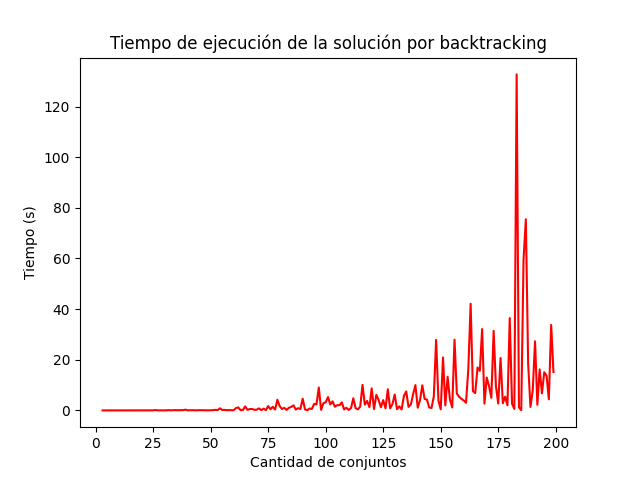
\includegraphics[width=0.6\textwidth]{graficos/backtracking.png}
\end{figure}

En la gráfica anterior se observan los tiempos de ejecución para la implementación usando backtracking, es importante destacar la gran variabilidad entre los tiempos de ejecución existentes entre los conjuntos. Esto se debe a la variabilidad que existe entre los conjuntos con los cuales se va probando en cada paso el algoritmo 

\subsection{Tiempos de ejecución por Programación Entera}

\begin{figure}[H]
    \centering
    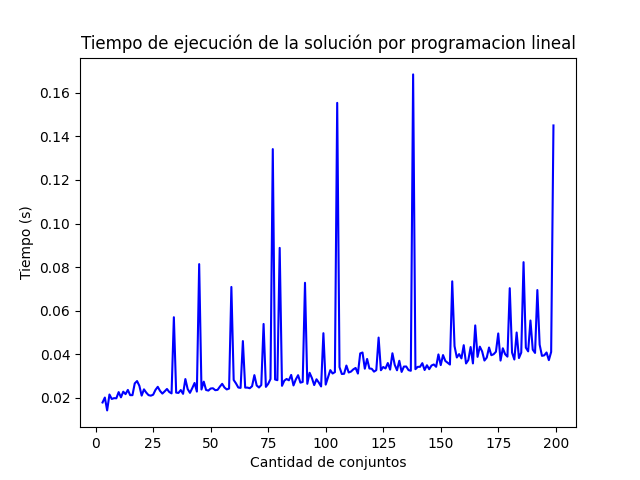
\includegraphics[width=0.6\textwidth]{graficos/integerp.png}
\end{figure}

Por otro lado los tiempos de ejecución para la solución por programación lineal entera son más pequeños en comparación a la solución por backtracking. Debido al uso de la biblioteca \textbf{pulp} se estima que dicha resolución cuenta con optimizaciones ocultas al desarrollador y por lo tanto pareciera que la tendencia temporal tiende a ser algo lineal 

\subsection{Comparación entre ambos métodos}

Finalmente se grafican sobre una misma escala ambos métodos y se aprecia la amplia diferencia entre ambos

\begin{figure}[H]
    \centering
    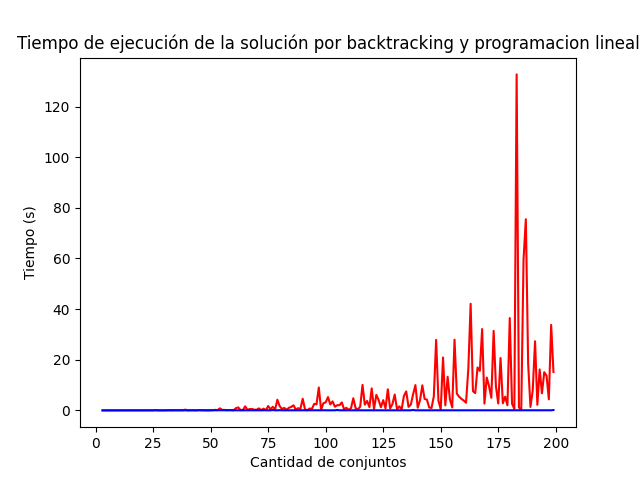
\includegraphics[width=0.6\textwidth]{graficos/ilpvsbt.png}
\end{figure}

\section{Estimación contra cota teórica}

\subsection{Backtracking acotado por curva teórica}

Se genero una gráfica con una curva teórica exponencial, con lo cual se puede apreciar que la implementación por backtracking se comporta efectivamente de manera exponencial al conjunto de entrada 

\begin{figure}[H]
    \centering
    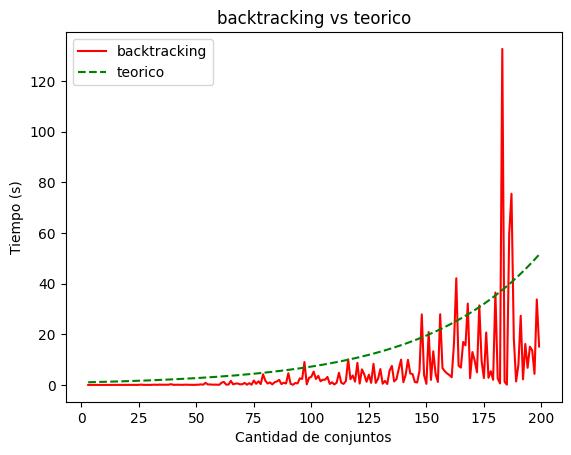
\includegraphics[width=0.6\textwidth]{graficos/backvsteorico.png}
\end{figure}

\section{Construyendo aproximaciones}

\subsection{Solución Greedy}

Como es sabido el Hitting Set Problem pertenece a NP-completo y por lo tanto no existe ninguna solución que de en tiempo polinomial de una respuesta exacta en todo caso posible, pero, es posible construir una aproximación a la solución utilizando una estrategia greedy

\subsubsection{La estrategia}

Para construir una aproximación greedy se deben cumplir las siguientes reglas:

\begin{itemize}
    \item Aplicar una regla sencilla \\
    \item Debe conseguir un óptimo local al problema actual \\
    \item Se deben repetir estas reglas hasta conseguir una respuesta \\
\end{itemize}

Por lo tanto se construye la siguiente estrategia greedy para resolver el problema:

\begin{itemize}
    \item Conseguir el jugador más representativos cuya frecuencia de aparición es la más alta entre todos los jugadores \\
    \item Eliminar todos los subconjuntos en donde este jugador aparezca \\
    \item Repetir hasta que no quede ningún subconjunto de jugadores \\
\end{itemize}

\subsubsection{La implementación}

Siguiendo los pasos anteriormente mencionados se construye la implementación en python del algoritmo de aproximación greedy 

\begin{lstlisting}[language=Python, caption= aproximación greedy, label=python_code]
def aprox_hs_by_greedy(subsets: set, a: set):
    aprox_sol = set()
    missing_sets = set(range(len(subsets)))
    subsets = list(subsets)
    return _aprox_greedy(subsets, aprox_sol, missing_sets)

def _aprox_greedy(subsets: list, aprox_sol: set, missing_sets: set):
    while(not is_solution(aprox_sol, subsets)):
        diference = set()
        player = find_most_frequent_player(missing_sets, subsets)
        for i in missing_sets: 
            if has_a_player(subsets[i], player):
                diference.add(i)
        aprox_sol.add(player)
        missing_sets.difference_update(diference)
    return aprox_sol

def find_most_frequent_player(missing_sets: set, subsets: list):
    frequency = dict()
    for subset_index in missing_sets:
        for player in subsets[subset_index]:
            frequency[player] = frequency.get(player, 0) + 1
    most_frequent_player = max(frequency, key=frequency.get)
    return most_frequent_player
\end{lstlisting}

\subsubsection{Complejidad temporal}

Para analizar la complejidad temporal del algoritmo vemos que se hacen las siguientes iteraciones sobre el algoritmo: 

\begin{enumerate}
    \item Se busca al jugador más frecuente, esto es recorre $m$ subconjuntos y por cada uno de ellos sus $k$ jugadores\\
    \item Se ejecuta un ciclo while, que en el peor de los casos realiza $m$ iteraciones y en cada una de esas realiza la llamada a buscar el jugador más frecuente
\end{enumerate}

Por lo tanto se puede concluir que el algoritmo tiene la siguiente complejidad:

$$
    T(n) = O(m^2 \cdot k)
$$
Donde $k$ se puede estimar como el cardinal del mayor subconjunto perteneciente a $m$ y $m$ como el cardinal de $m$. Importante destacar que esta cota corresponde al peor caso posible y el algoritmo podría comportarse mejor de lo esperado dependiendo de la cantidad de jugadores que necesite $k$

\subsection{Solución por programación lineal}

Para construir esta aproximación se relajan las reglas implementadas en el caso de programación lineal entera y se permite que los valores de los jugadores varíen entre 0 y 1. Por lo que las ecuaciones en este caso serían:
\begin{align}
  \sum_{b_j \in B_i} b_j &\geq 1 \quad \forall B_i \in B \\
  \sum_{b_j \in B_i} b_j &\geq 1 \quad \forall B_i \in B \\
  b_j &\in [0,1] 
\end{align}
\subsubsection{Complejidad temporal de la aproximación}
Debido a que se esta aproximación se realiza aplicando programación lineal, es claro que, para resolver las ecuaciones planteadas se utiliza el algoritmo Simplex, el cual, se encuentra acotado como:
\begin{align}
    T(n) = O(n^9)
\end{align}
Si bien es cierto que se pueden dar determinadas condiciones para que la complejidad temporal de la resolución aproximada sea menor a la anteriormente mencionada, no se puede descartar que algoritmo Simplex que es el motor de la solución posee la cota superior dicha 
\subsubsection{Clasificación de la aproximación}
Definamos $M$ como el subconjunto con la cantidad máxima de jugadores y definamos $|M| = b$ si se desean relajar las ecuaciones y establecer que dentro de las respuesta vayan solo los elementos cuya respuesta en la solución es: $1/b$. En el peor de los casos para todos los elementos de ese subconjunto todos los valores en la ecuación pueden tomar $1/b$, aunque también, eso quiere decir que todos los valores estarían incluidos. Como $1/b$ es un valor pequeño en comparación a los posibles valores que puedan tomar los otros jugadores dentro de sus ecuaciones, recordar que la suma de jugadores por cada subconjunto debe valer al menos uno, para otros conjuntos es probable también se incluyan otros valores que no son necesarios en la respuesta óptima. Por lo tanto, volviendo a $|M|$, se observa que como mucho necesita un representante, es cierto que, pueden existir dentro de $M$ la presencia de otros jugadores esenciales en la respuesta óptima pero en un principio en el peor caso se incluyen $b - 1$ jugadores no esenciales, entonces, esto es una $b - 1$ aproximación
\subsubsection{Una muestra de r(A)}

A continuación se toma una muestra aleatoria de los $r(A)$ de la solución
\begin{table}[H]
    \centering
    \begin{tabular}{cc}
    \hline
    \textbf{m} & \textbf{r(a)} \\
    \hline
    104 & 1.875000 \\
    15 & 1.000000 \\
    152 & 1.181818 \\
    196 & 1.700000 \\
    150 & 1.300000 \\
    16 & 1.000000 \\
    161 & 1.000000 \\
    66 & 1.000000 \\
    27 & 1.400000 \\
    95 & 1.000000 \\
    115 & 2.142857 \\
    153 & 1.076923 \\
    92 & 2.125000 \\
    112 & 1.900000 \\
    35 & 1.000000 \\
    135 & 1.000000 \\
    45 & 3.000000 \\
    96 & 2.000000 \\
    19 & 3.000000 \\
    163 & 1.600000 \\
    \hline
    \end{tabular}
    \caption{Descripción de la tabla.}
    \label{tabla:resultados}
\end{table}

\subsection{Medición de las aproximaciones}
\begin{figure}[H]
    \begin{minipage}{0.5\textwidth}
        \centering
        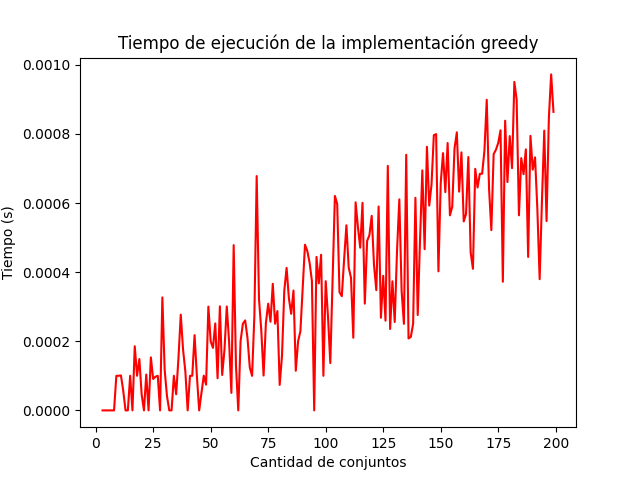
\includegraphics[width=\linewidth]{graficos/greed.png}
        \caption{Aproximación greedy}
        \label{fig:imagen1}
    \end{minipage}%
    \begin{minipage}{0.5\textwidth}
        \centering
        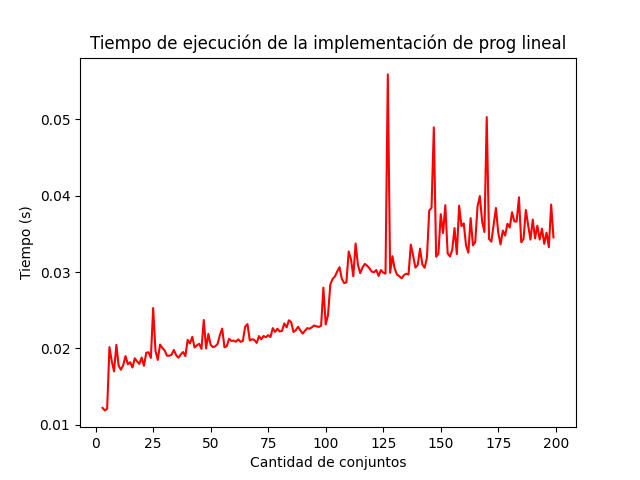
\includegraphics[width=\linewidth]{graficos/continous.png}
        \caption{Aproximación por prog. lineal}
        \label{fig:imagen2}
    \end{minipage}
\end{figure}

En las gráficas anteriores se puede observar la duración en microsegundos para el mismo set de datos utilizado a la hora de tomar mediciones sobre las soluciones exactas al problema. Se observa que la solución greedy posee una variabilidad mayor entre valores de $m$, a comparación de la solución por programación lineal que se mantiene mas estable entre los diferentes tamaños de $m$

\subsection{Comparación entre los tamaños de los óptimos}

En el siguiente gráfico se podrán observar los valores de los óptimos resultantes de ambas aproximaciones y el óptimo arrojado por una de las soluciones exactas, es fácilmente apreciable que, la aproximación por un algoritmo greedy es la cual posee el menor error a la hora de aproximar. Al mismo tiempo, se aprecia que la aproximación realizada por programación lineal no se perfila como una buena aproximación a utilizar 

\begin{figure}[H]
    \centering
    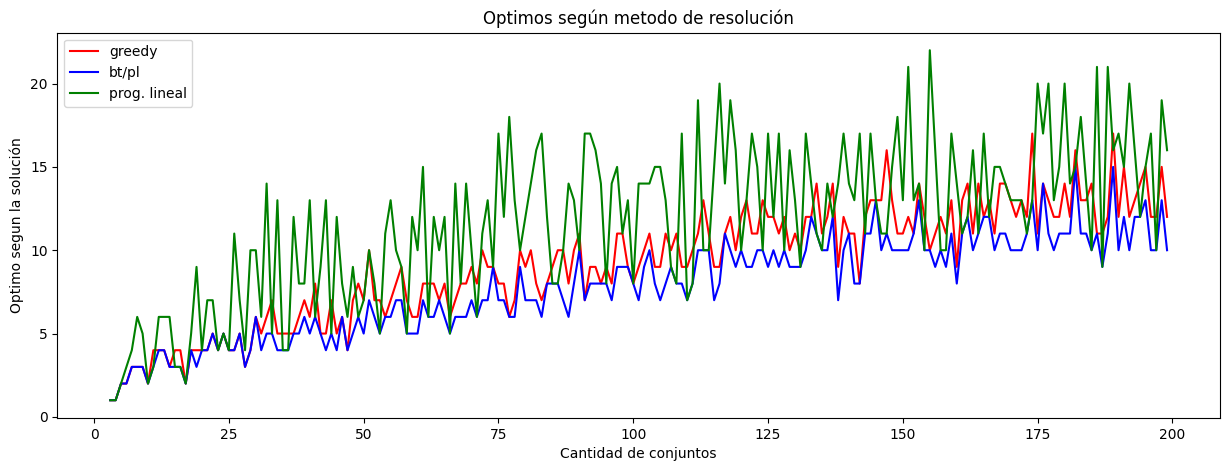
\includegraphics[width=1\textwidth]{graficos/optimos.png}
\end{figure}

En este gráfico se analizan las distancias con el óptimo real de ambas aproximaciones, confirmando una vez más que la aproximación por el algoritmo greedy tiende a distar menos del óptimo real, siendo la máxima distancia al óptimo de 5 elementos 

\begin{figure}[H]
    \centering
    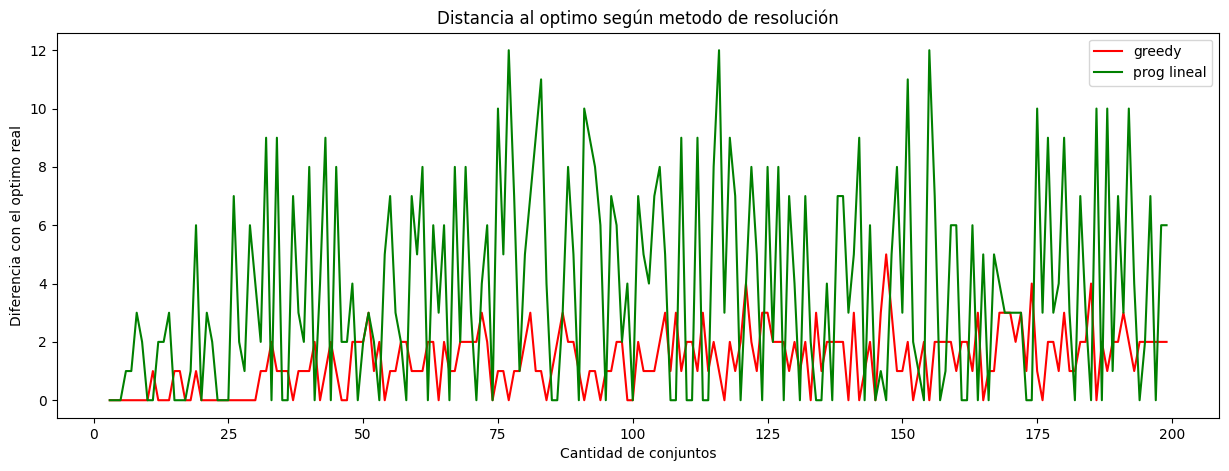
\includegraphics[width=1\textwidth]{graficos/distanciaaloptimo.png}
\end{figure}

\subsection{Mediciones en volumen de las aproximaciones}
\begin{figure}[H]
    \begin{minipage}{0.5\textwidth}
        \centering
        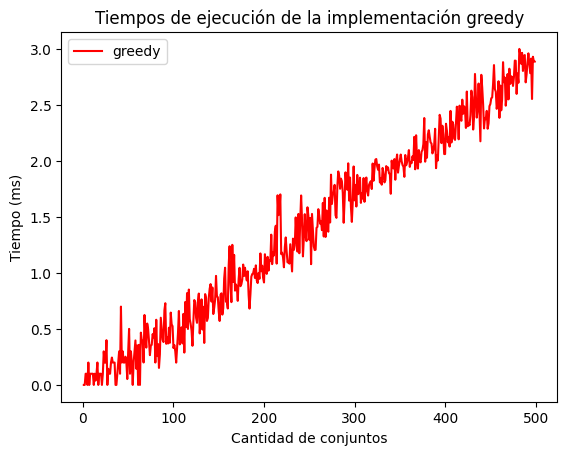
\includegraphics[width=\linewidth]{graficos/greedvol.png}
        \caption{Tiempo en vol. por greedy}
        \label{fig:imagen1}
    \end{minipage}%
    \begin{minipage}{0.5\textwidth}
        \centering
        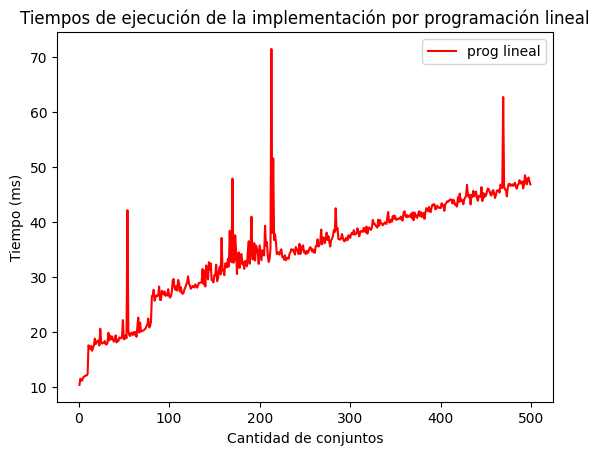
\includegraphics[width=\linewidth]{graficos/plvol.png}
        \caption{Tiempo en vol. por prog. Lineal}
        \label{fig:imagen2}
    \end{minipage}
\end{figure}
\section{Conclusión}

En conclusión se analizo en profundidad un análisis y diversas resoluciones del problema de conjunto de impacto, construyendo tanto estrategias que permitían obtener una solución exacta como aproximaciones diversas aproximaciones que varían en comportamiento y complejidad temporal es importante destacar lo siguiente:

\begin{itemize}
    \item La aproximación por programación lineal tuvo menor variabilidad entre los tiempos de ejecución que la solución aproximada por una estrategia greedy a pesar de tener una complejidad temporal menor\\
    \item La aproximación greedy genera óptimos más cercanos a los reales para cualquier valor tamaño del conjunto de subconjuntos siendo pues que para los datos utilizados para resolver todos los algoritmos implementados la mayor distancia al óptimo fue 6 \\
    \item La solución por programación lineal entera encuentra con los mejores tiempos entre todos los algoritmos la respuesta \\ 
\end{itemize}
\end{document}